\documentclass[12pt]{article}
\usepackage{url,amsmath,amsthm,enumitem,amsfonts,tikz,verbatim,amssymb, wasysym, clrscode3e, booktabs, soul}
% \usepackage[doublespacing]{setspace}
\usepackage[makeroom]{cancel}
\usepackage{natbib}
\usepackage{graphicx}
\usepackage{listings}
\usetikzlibrary{arrows}

\title{ University of Massachusetts Lowell \protect\\
	Department of Mathematical Sciences\protect\\
MATH 4750 \protect\\
Senior Seminar Project Report}
\author{Joel Savitz \\ Fall 2020 \\ SID: 01739537}

\lstset
{
    %Formatting for code in appendix
    showstringspaces=false,
    breaklines=true,
    breakatwhitespace=false,
}

\newcommand{\reals}{\mathbb{R}}

\begin{document}

\maketitle

\begin{abstract}
	In this paper,
	I verify Newton's law of cooling my experimentation
	using cheap and widely available sensors and devices
	and free and open source software systems.
	I find that the law is hold for this system,
	and describe my particular system
	with a differential equation
	that contains a numerically calculated cooling coefficient.
\end{abstract}

\section{Introduction}

Scientists express physical laws of
the universe in the language of differential equations.
The reason for this is not immediately obvious,
though my personal work with differential equations
has provided me with an intuition as to why.
Fortunately for me,
one scientist describes three necessary properties
of a physical law that are satisfied by a differential equation as: 


\begin{itemize}
	\item ``The mathematical relation must be sufficiently general"
	\item ``It must define connections between neighboring points"
	\item ``It must imply the continuity of change"\citep{whydiffeq}
\end{itemize}

Differential equations satisfy all three of these properties
since they are general enough that
changes to the initial values of a system
do not violate the constraints defined by a general solution
and the relationship between a function and one or more of its derivatives
defines the connection between points in the domain of the function
and implies that change in the system is continuous
due to the nature of calculus.


Newton's law of cooling states that
``the rate of heat loss of a body is
directly proportional to the difference
in the temperatures between the body and
its surroundings" \citep{wiki}.

Let $\Delta T$ be the difference between
the temperature of the body
and the ambient temperature of the environment
as a function of a point in time $t$,
we have that equation \ref{eq1}
describes Newton's law of cooling.

\begin{align} \label{eq1}
	\frac{d\Delta T}{dt} = k\Delta T(t) \textrm{ for some $k \in \reals$}
\end{align}

Then, we can solve this differential equation by separating the parameters.

\begin{align} \label{eq2}
	\frac{dT}{dt}\frac{1}{\Delta T(t)} & = k \\
	\int \frac{dT}{dt}\frac{1}{\Delta T(t)} dt & = \int k dt \\
	\ln|\Delta T(t)| & = kt + C \textrm{ for some $C \in \reals$} \\
	e^{\ln | \Delta T(t) | } = & e^{kt + C} \\
	\label{eq3}
	\Delta T(t) = & De^{kt} \textrm{ where $D = e^C$ }
\end{align}

In this paper, I verify the this law
relative to a particular environment
and calculate an approximate value of the cooling coefficient
by fitting experimental data to equation \ref{eq3}.

\section{Materials and Methods}

I performed this experiment using
using a hardware sensor
to a Raspberry Pi computer,
specifically the model 4B+ with 8GB of RAM.

I purchased the DS18D20,
a waterproof temperature sensor compatible with the Raspberry Pi.
These sensors are relatively inexpensive,
and I purchased a 5 pack for $\$12.98$ on Amazon \citep{Amazon}.

With the equipment in hand,
I set up the physical system
on a small table
where I had previously configured
my two raspberry pi computers.
I wired the sensors to the raspberry pi using
a breadboard, as seen in figure \ref{fig3}.

As you can see in \ref{fig2},
the system lies under my air conditioner
set to cool my room to 70 degrees Fahrenheit.
Primarily, this was to keep my room comfortable,
but the additional cooling source added
a bit of noise to the data
that made the experiment a bit more interesting.

To prepare the system,
I simply filled a mug with tap water
and placed it in the microwave
for about a minute.
Then, as seen in figure \ref{fig2},
I placed one of the temperature sensors
inside of the water
and another right next to it,
hanging over the side of the mug,
to measure ambient temperature.

\begin{figure}
	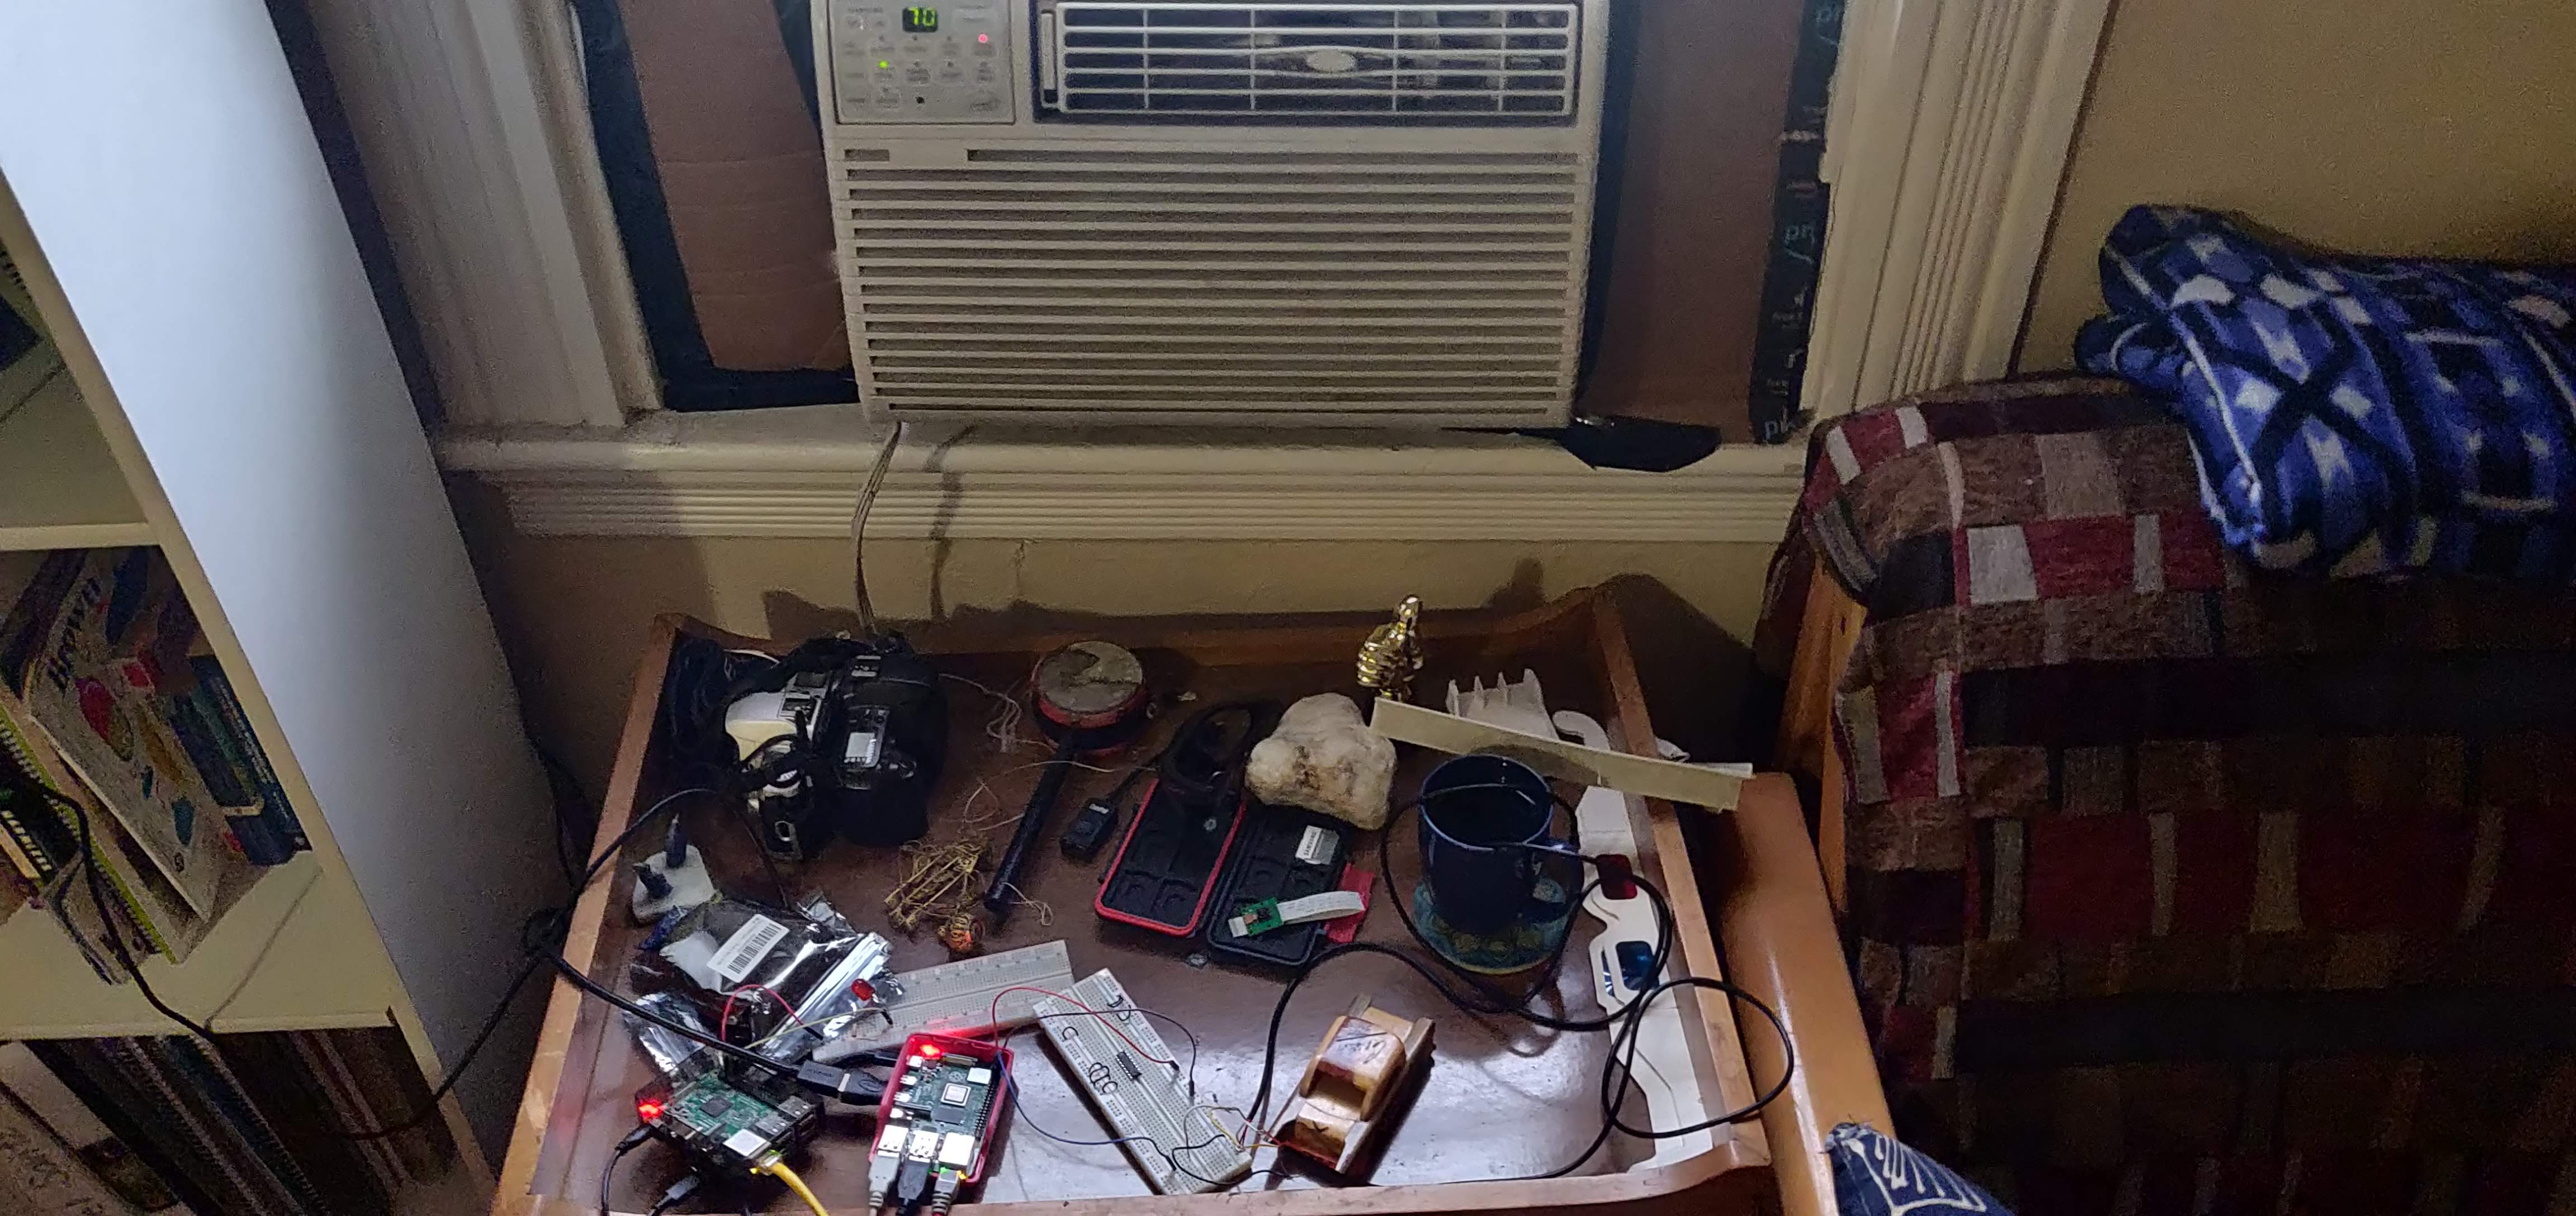
\includegraphics[scale=0.1]{full_setup.jpg}
	\centering
	\label{fig2}
	\caption{The full experimental setup}
\end{figure}

\begin{figure}
	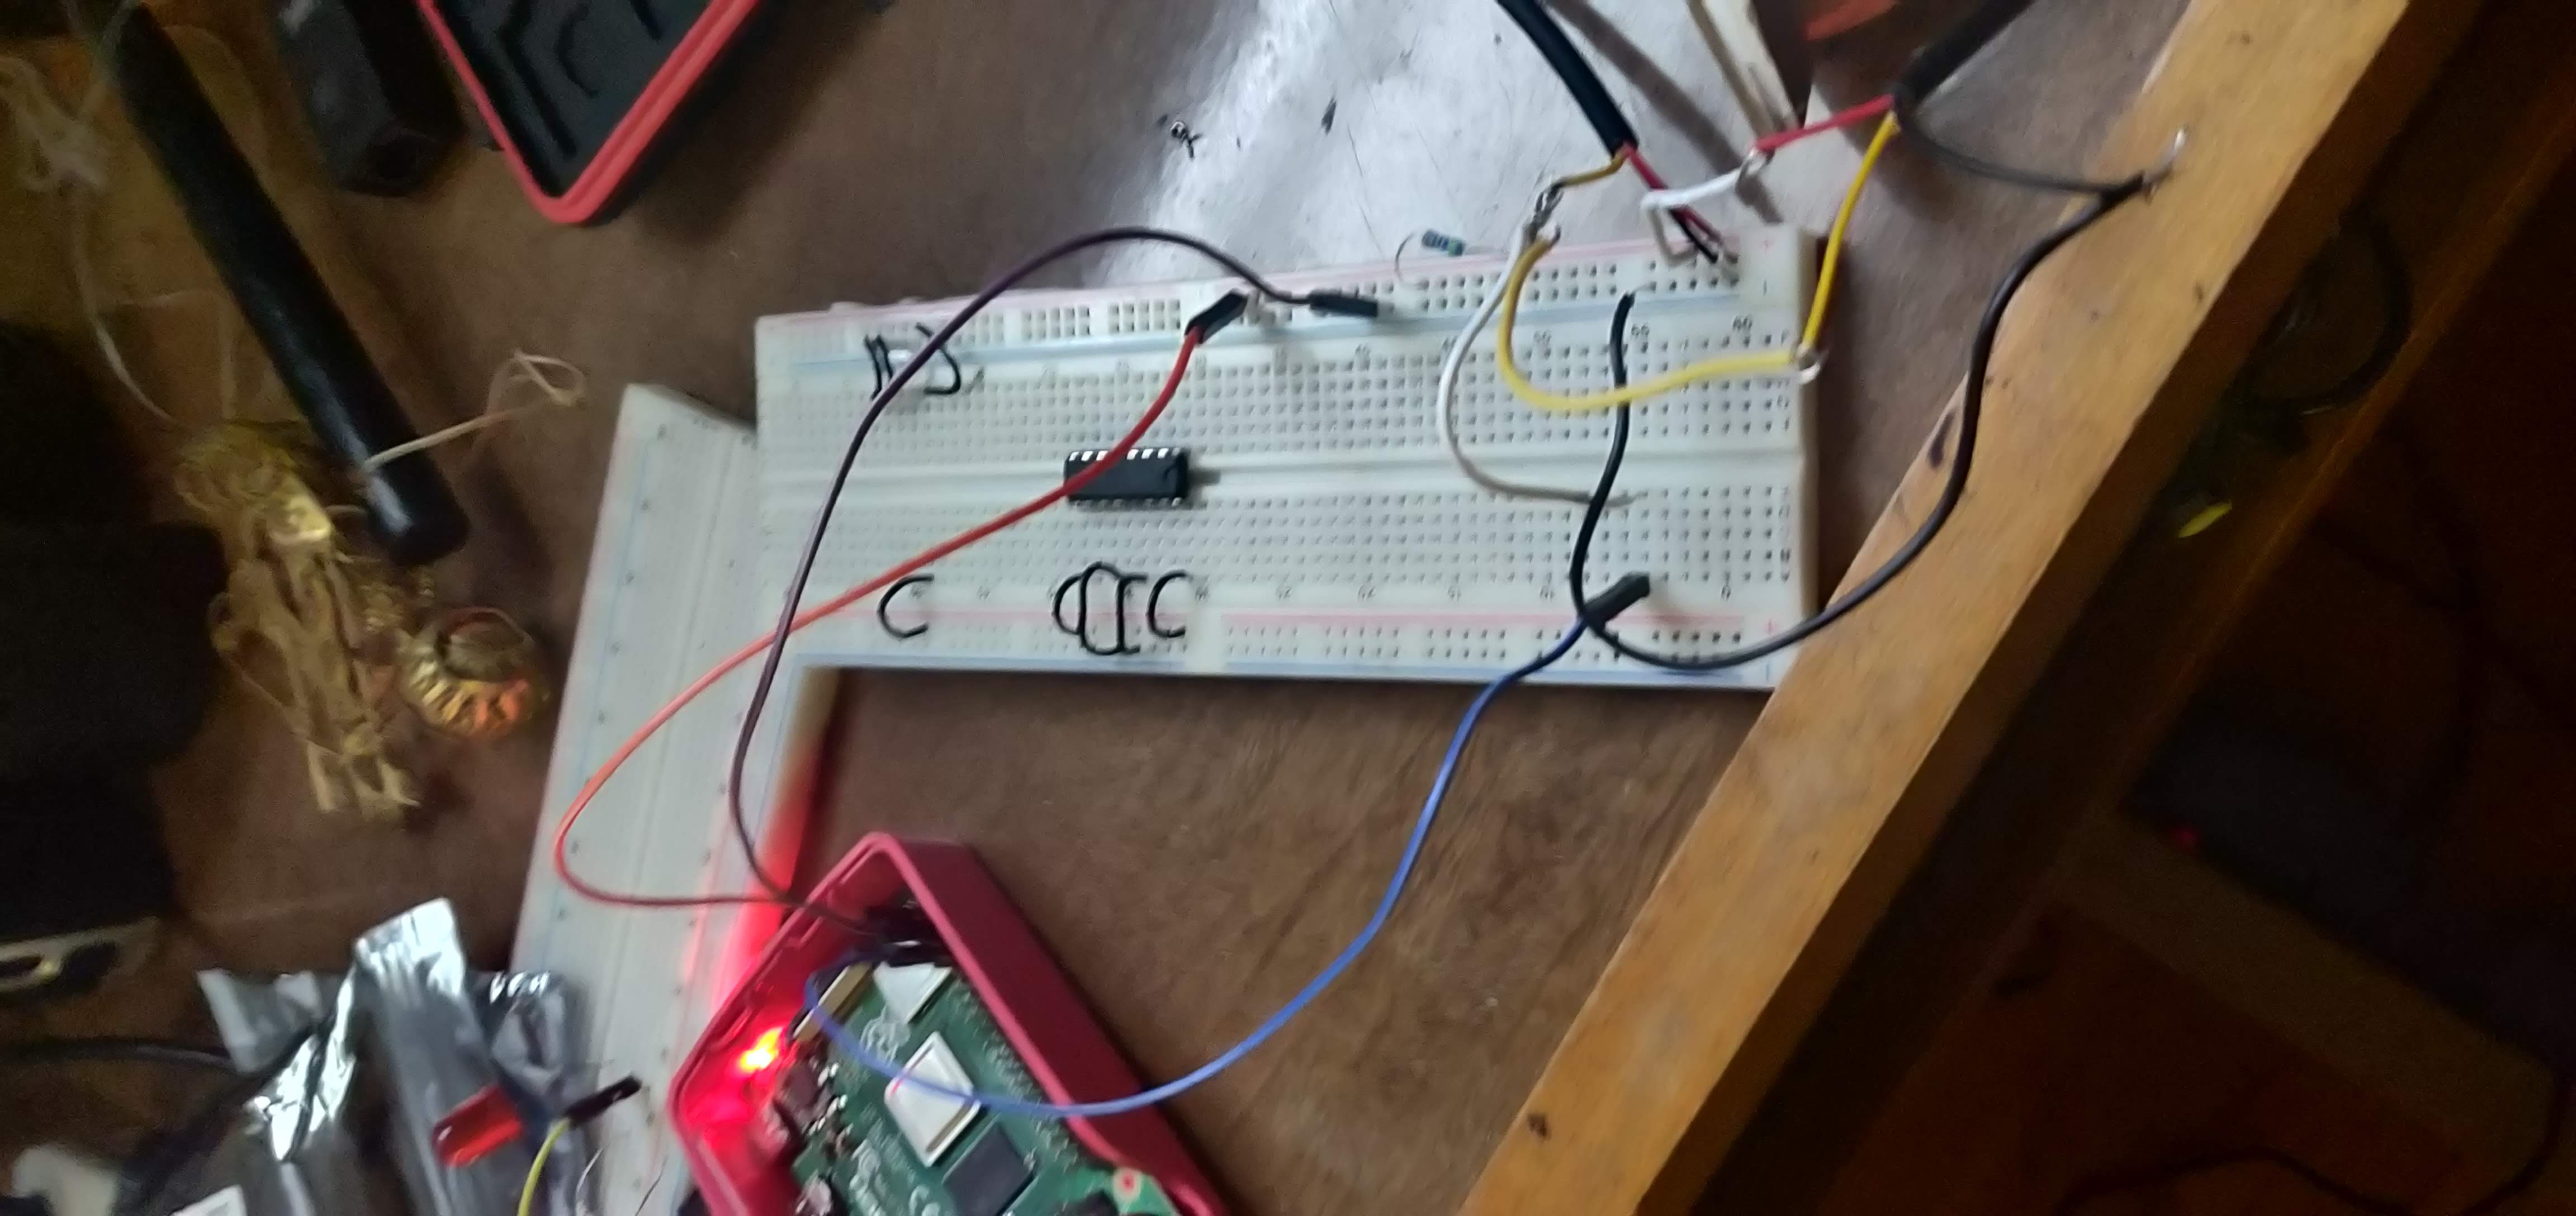
\includegraphics[scale=0.1]{wiring.jpg}
	\centering
	\label{fig3}
	\caption{A close up of the wiring}
\end{figure}

I wrote two software programs for this experiment,
the first to gather the data,
and the second to perform analysis on it.
For this reason, the first program
is called \texttt{gather},
and the second program is called \texttt{analysis}.
See sections \ref{apxA} and \ref{apxB} for the full code listings.


\section{Results}

The sensors gathered the data
for just over 4 hours.
The full dataset is accessible
in the project git repository
as the file \texttt{gather/data2} \cite{project_repo}.
As seen in figure \ref{fig1},
the raw data contained
a sharp oscillating pattern
as the difference between
the temperature of the body
and the ambient temperature
of the surrounding environment
decayed towards zero.
I suspect this was due
to the thermostat of the nearby air conditioner
turning off and on in order to maintain the room temperature.
Regardless of this fluctuation,
the data displayed a clear trend
of exponential decay,
validating and confirming
Newton's law of cooling.

Using non-linear least squares regression,
courtesy of the \texttt{scipy} python library,
I was able to find a curve of best fit,
and approximate the following equation for this system:

\begin{align}
	\Delta T(t) = 26.31e^{-3.658 \times 10^{-4} t} - 0.4938
\end{align}

Thus the approximate value of the cooling coefficient,
denoted $k$ in equation \ref{eq3},
is $3.658 \times 10^{-4}$,
and we can write the following differential equation
to approximate this system:

\begin{align}
	\frac{d\Delta T}{dt} = 3.658 \times 10^{-4}\Delta T(t)
\end{align}

\begin{figure}
	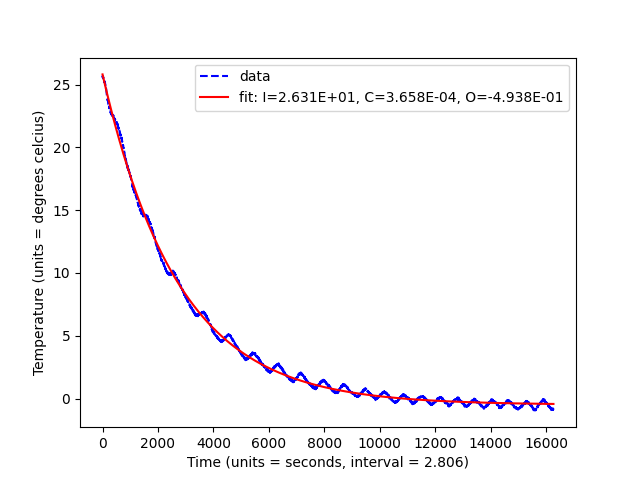
\includegraphics[scale=0.8]{Figure_1.png}
	\centering
	\label{fig1}
	\caption{A plot of the data and the fitted curve}
\end{figure}

\section{Discussion}

For this relatively small difference
between the temperature of a cup of hot water
and my room with a running and fairly powerful 10,000 BTU air conditioner,
Newton's law of cooling approximates
the rate at which the temperate of the body of concern
decays to the temperature of its environment.
This is a testament to the genius of Isaac Newton,
whose scientific articulation was able to describe
the behavior of a cup of water in my room
several hundred years in advance.

Using my small software suite
and relatively inexpensive equipment,
I could replicate this experiment
on a wide variety of systems,
given that the temperatures of concern
are within the detection range of the sensors
and the operating temperature of the nearby
raspberry pi computer.
In a small but significant sense,
this experiment demonstrates the democratization of the scientific process,
for almost anyone could acquire the same equipment,
and perhaps using my freely available software,
replicate my experiment and validate Newton's law for themselves.
The beauty of scientific and mathematical progress and discovery
lies in its objective nature.
This physical law describes the behavior of physical systems
whether a person believes in their validity or not,
and the most skeptical mind may take matters into their own hands
and validate this equation as I have,
with no need to appeal to an authority other than nature itself.

\medskip
\noindent
The code listings of my \texttt{gather} and \texttt{analysis} programs follow as appendices.

\section{Appendix A: The \texttt{gather} program} \label{apxA}

\subsection{Main program}

\lstinputlisting[language=Python]{../gather/gather.py}

\subsection{Wrapper shell script}

\lstinputlisting[language=bash]{../gather/gather.sh}

\section{Appendix B: The \texttt{analysis} program} \label{apxB}

\lstinputlisting[language=Python]{../analysis/analysis.py}

\bibliographystyle{unsrtnat}
\bibliography{report}

\end{document}
